\documentclass{article}
\usepackage[utf8]{inputenc}
\usepackage[english]{babel}
\usepackage[font=small,labelfont=bf]{caption}
\usepackage{geometry}
\usepackage{natbib}
\usepackage{pxfonts}
\usepackage{graphicx}
\usepackage{newfloat}
\usepackage{setspace}
%\doublespacing

\newcommand{\argmax}{\mathop{\mathrm{argmax}}\limits}

\title{\textit{Supporting Information for: } High-level cognition during story listening is reflected in high-order dynamic correlations in neural activity patterns}
\author{Lucy L. W. Owen$^1$, Thomas H. Chang$^{1,2}$, and\
  Jeremy R. Manning\textsuperscript{$1, \dagger$}\\
  [0.1in]$^1$Department of Psychological and Brain
  Sciences,\\Dartmouth
  College, Hanover, NH\\
  $^2$Amazon.com, Seattle, WA\\
  \textsuperscript{$\dagger$}Address correspondence to
  jeremy.r.manning@dartmouth.edu}

\bibliographystyle{apa}

\begin{document}
\maketitle

\setcounter{equation}{0}
\setcounter{figure}{0}
\setcounter{table}{0}
\setcounter{page}{1}
\setcounter{section}{0}
\makeatletter
\renewcommand{\theequation}{S\arabic{equation}}
\renewcommand{\thefigure}{S\arabic{figure}}
\renewcommand{\bibnumfmt}[1]{[S#1]}
\renewcommand{\citenumfont}[1]{S#1}


\section*{Overview}
This document provides additional details and figures about the methods we used in the main text.

\begin{figure}[p!]
\centering
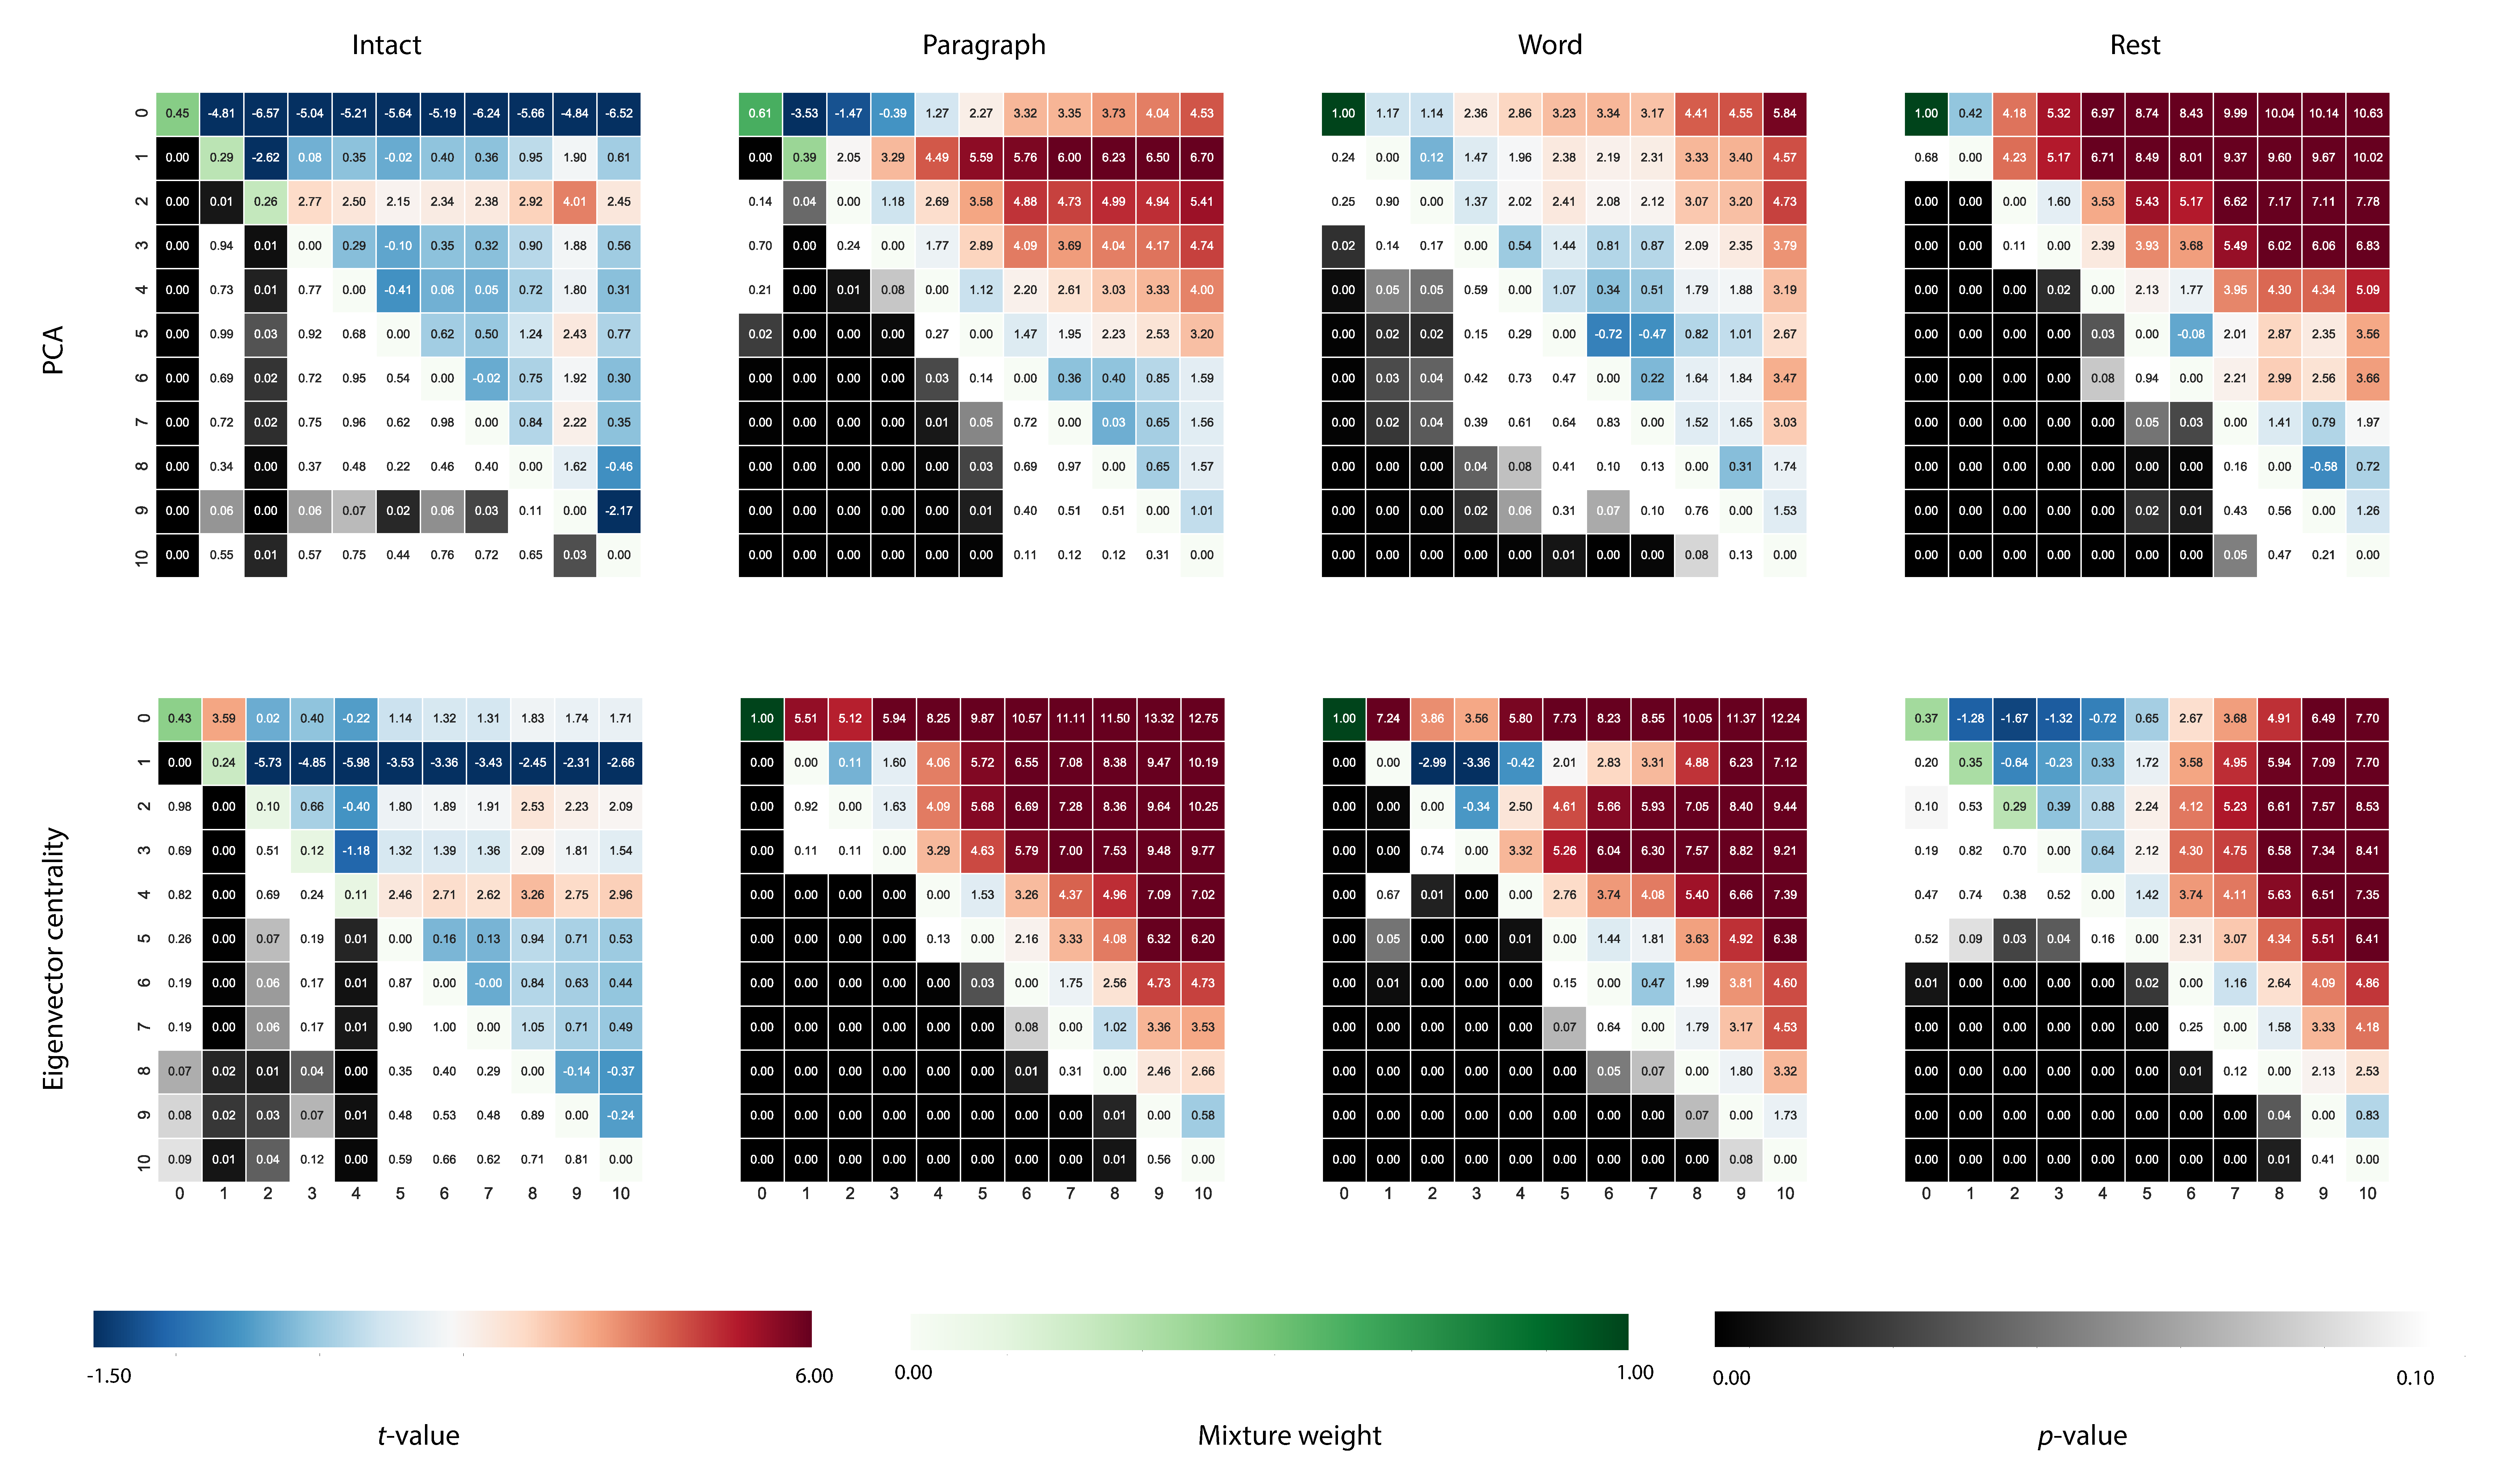
\includegraphics[width=1\textwidth]{figs/stats_heatmaps}
\caption{\small \textbf{Heatmaps conveying statistical results comparing decoding accuracy for each order.}  For each condition (intact, paragraph scrambled, word scrambled, and rest) and for each reduction technique (PCA and eigenvector centrality), we compared the distribution of decoding accuracy for each order. The upper triangle of each heatmap conveys the results of t-tests, and the lower triangle conveys corresponding p-values.  The diagonal is the results of the optimization of the phi parameter. }
\label{fig:stats_heatmaps}
\end{figure}

\begin{figure}[p!]
\centering
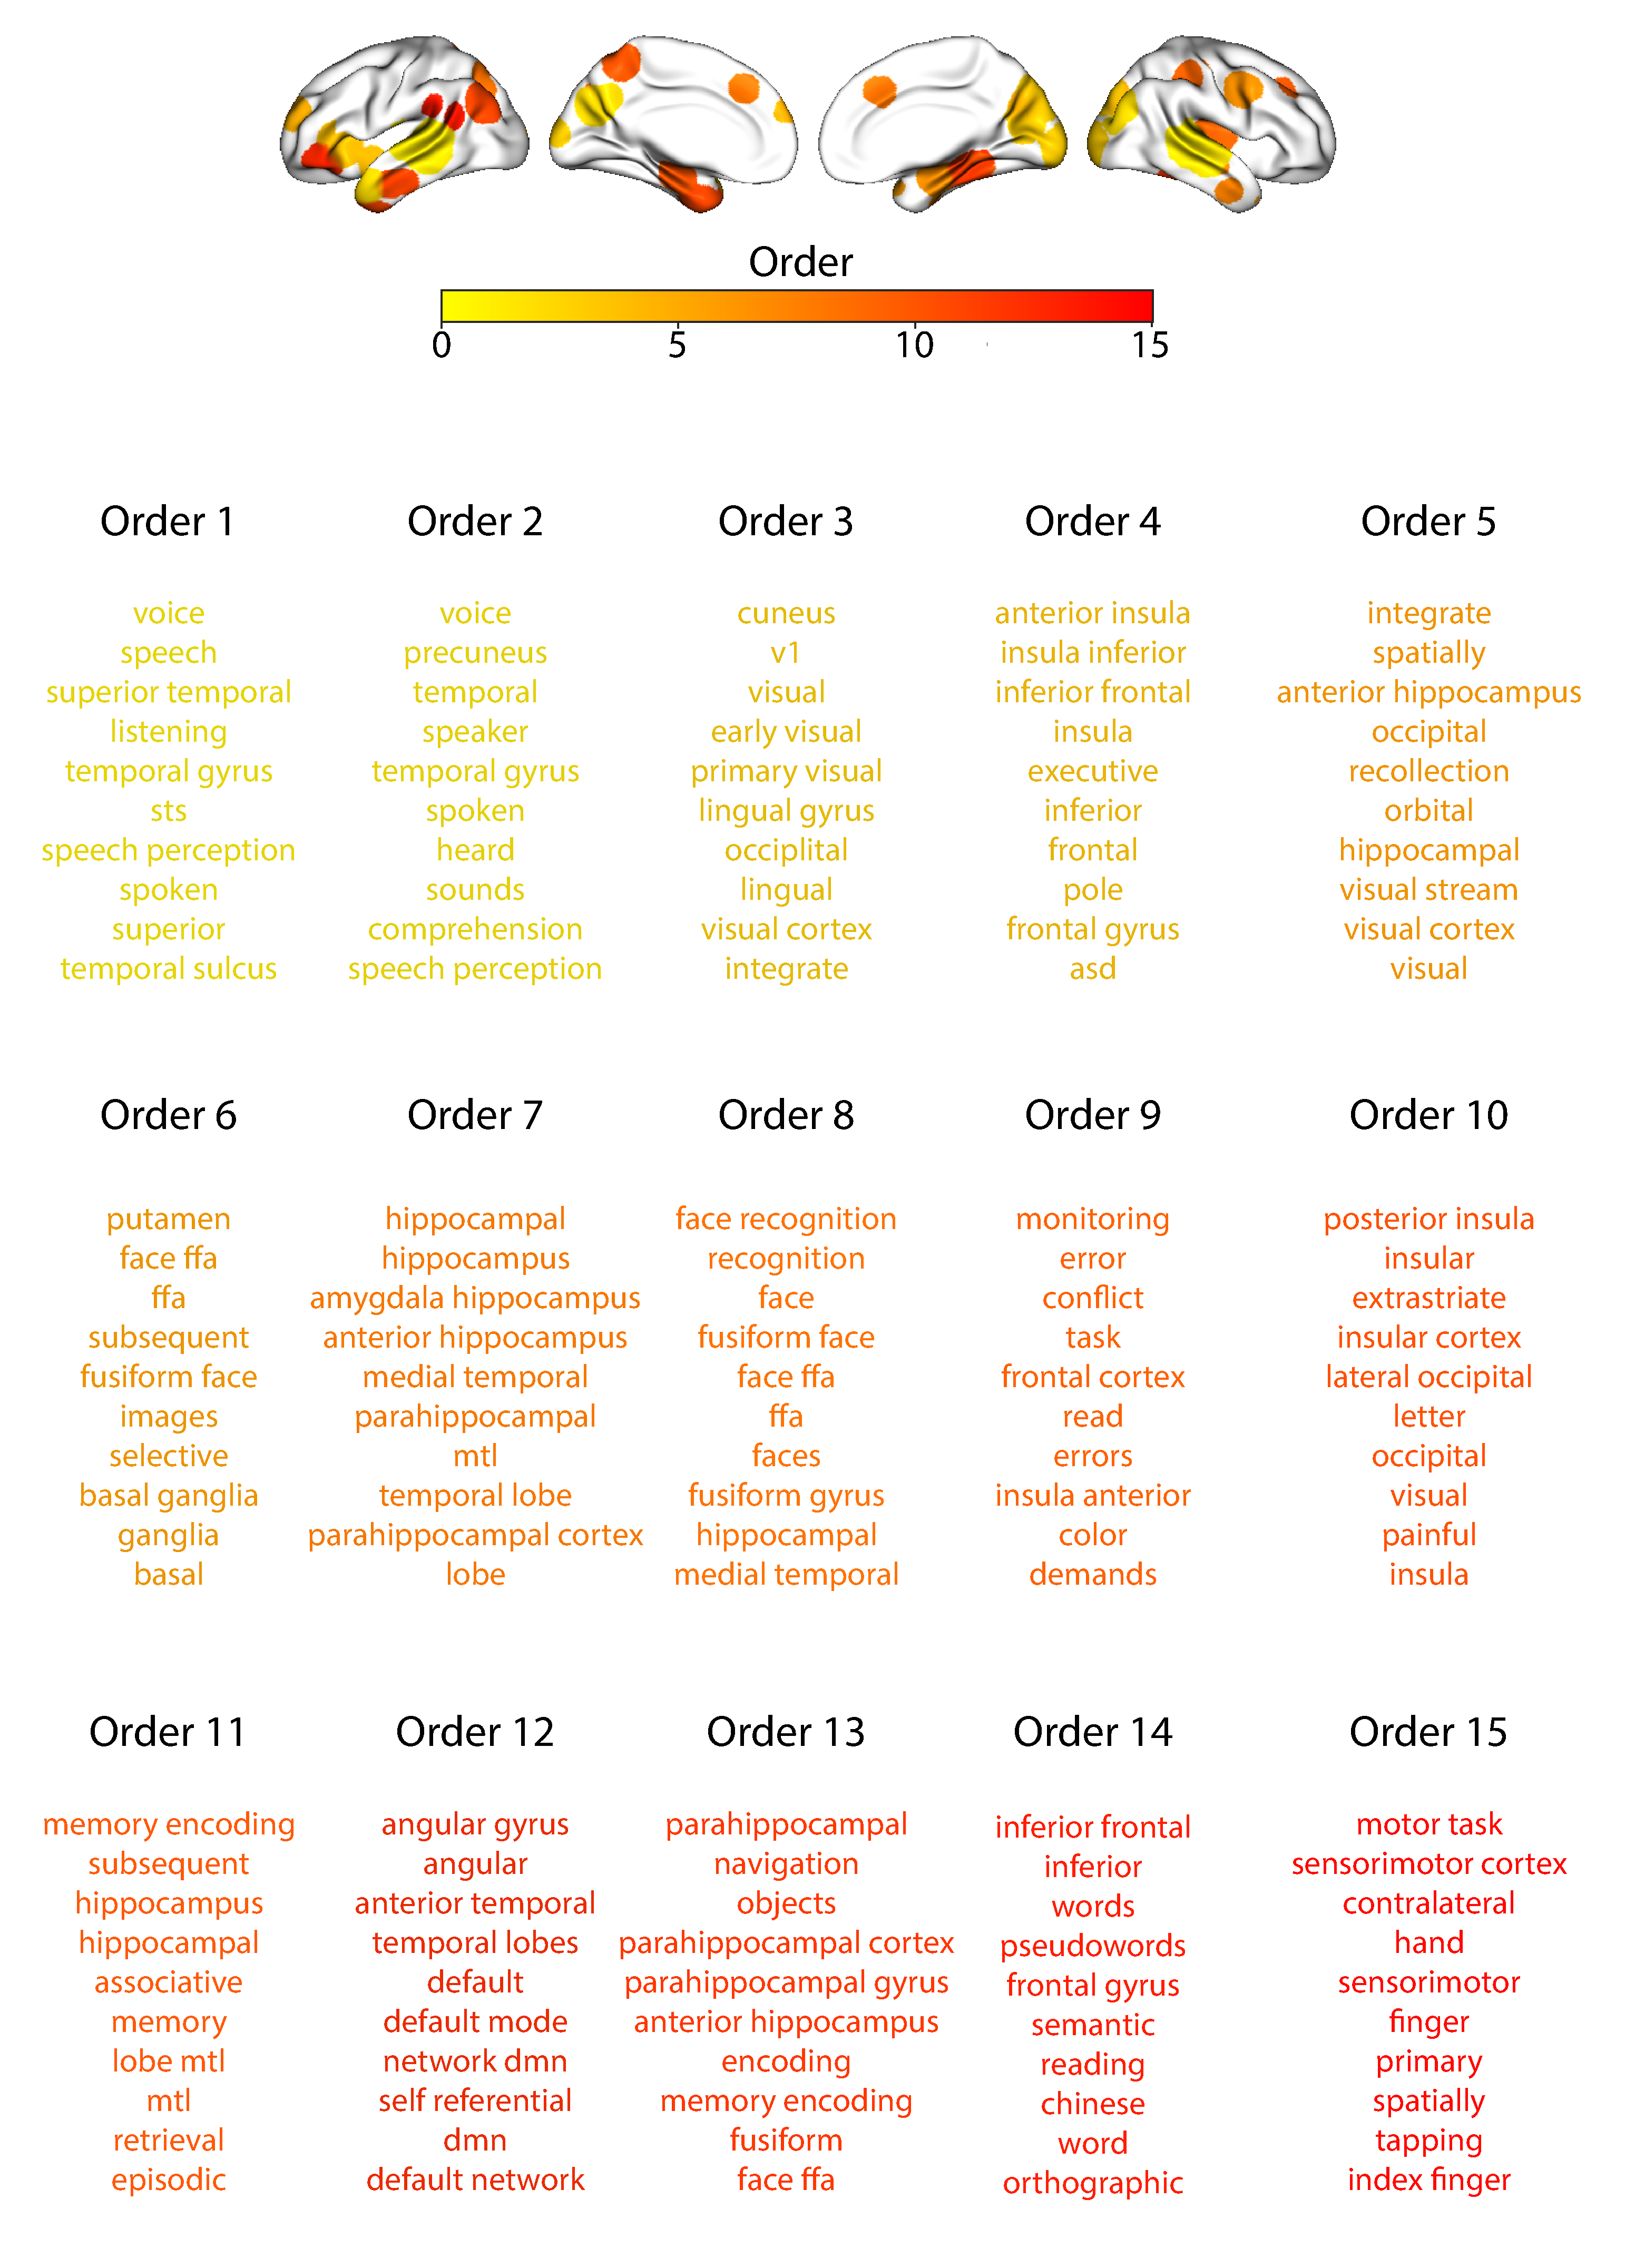
\includegraphics[width=\textwidth]{figs/supp_15_intact}
\caption{\small \textbf{Top 10 terms associated with the endpoints of the
      strongest correlations for the intact experimental condition.}  Each color corresponds to orders 1-15 of
    inter-subject functional correlations. The inflated brain plots
    display the locations of the endpoints of the 10 strongest
    (absolute value) correlations at each order, projected onto the
    cortical surface~\citep{CombEtal19}.  The lists of terms on the
    right display the top 10 Neurosynth terms~\citep{RubiEtal17}
    decoded from the corresponding brain maps for each order for the intact condition.}
\label{fig:intact}
\end{figure}

\begin{figure}[p!]
\centering
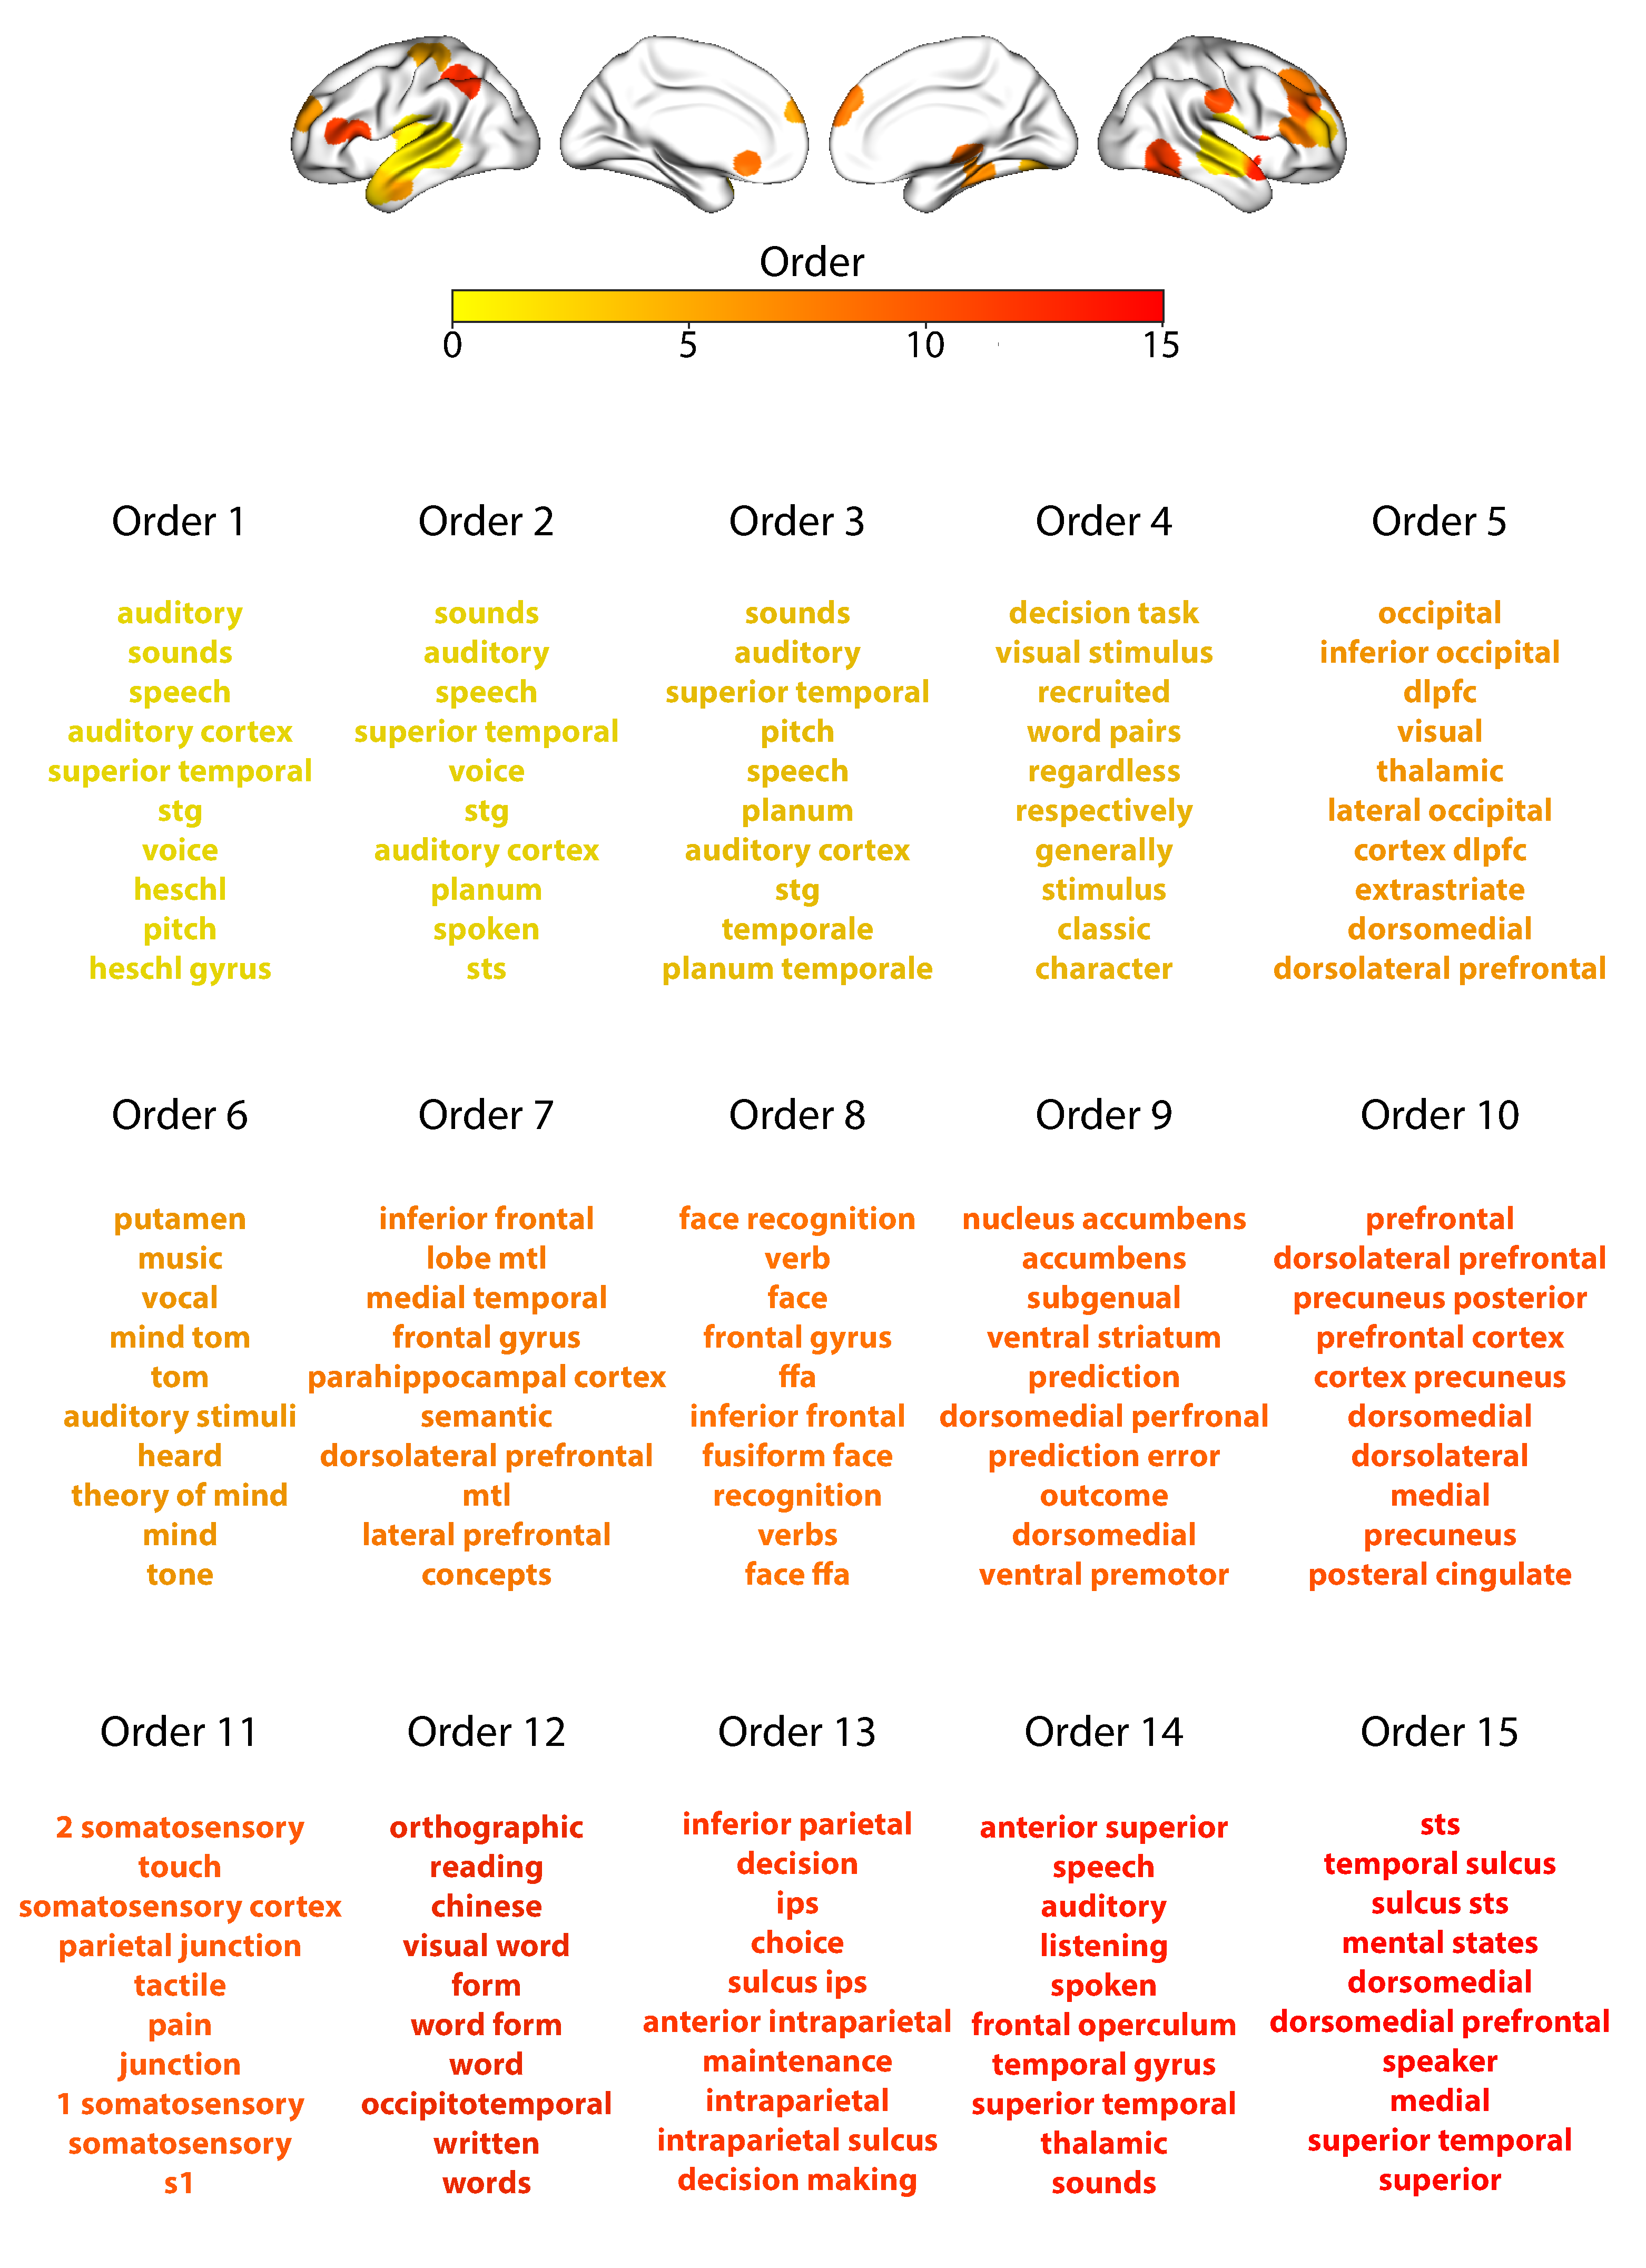
\includegraphics[width=\textwidth]{figs/supp_15_paragraph}
\caption{\small \textbf{Top 10 terms associated with the endpoints of the
      strongest correlations for the paragraph scrambled condition.}  Each color corresponds to orders 1-15 of
    inter-subject functional correlations for the paragraph scrambled condition. The inflated brain plots
    display the locations of the endpoints of the 10 strongest
    (absolute value) correlations at each order, projected onto the
    cortical surface~\citep{CombEtal19}.  The lists of terms on the
    right display the top 10 Neurosynth terms~\citep{RubiEtal17}
    decoded from the corresponding brain maps for each order.}
\label{fig:paragraph}
\end{figure}

\begin{figure}[p!]
\centering
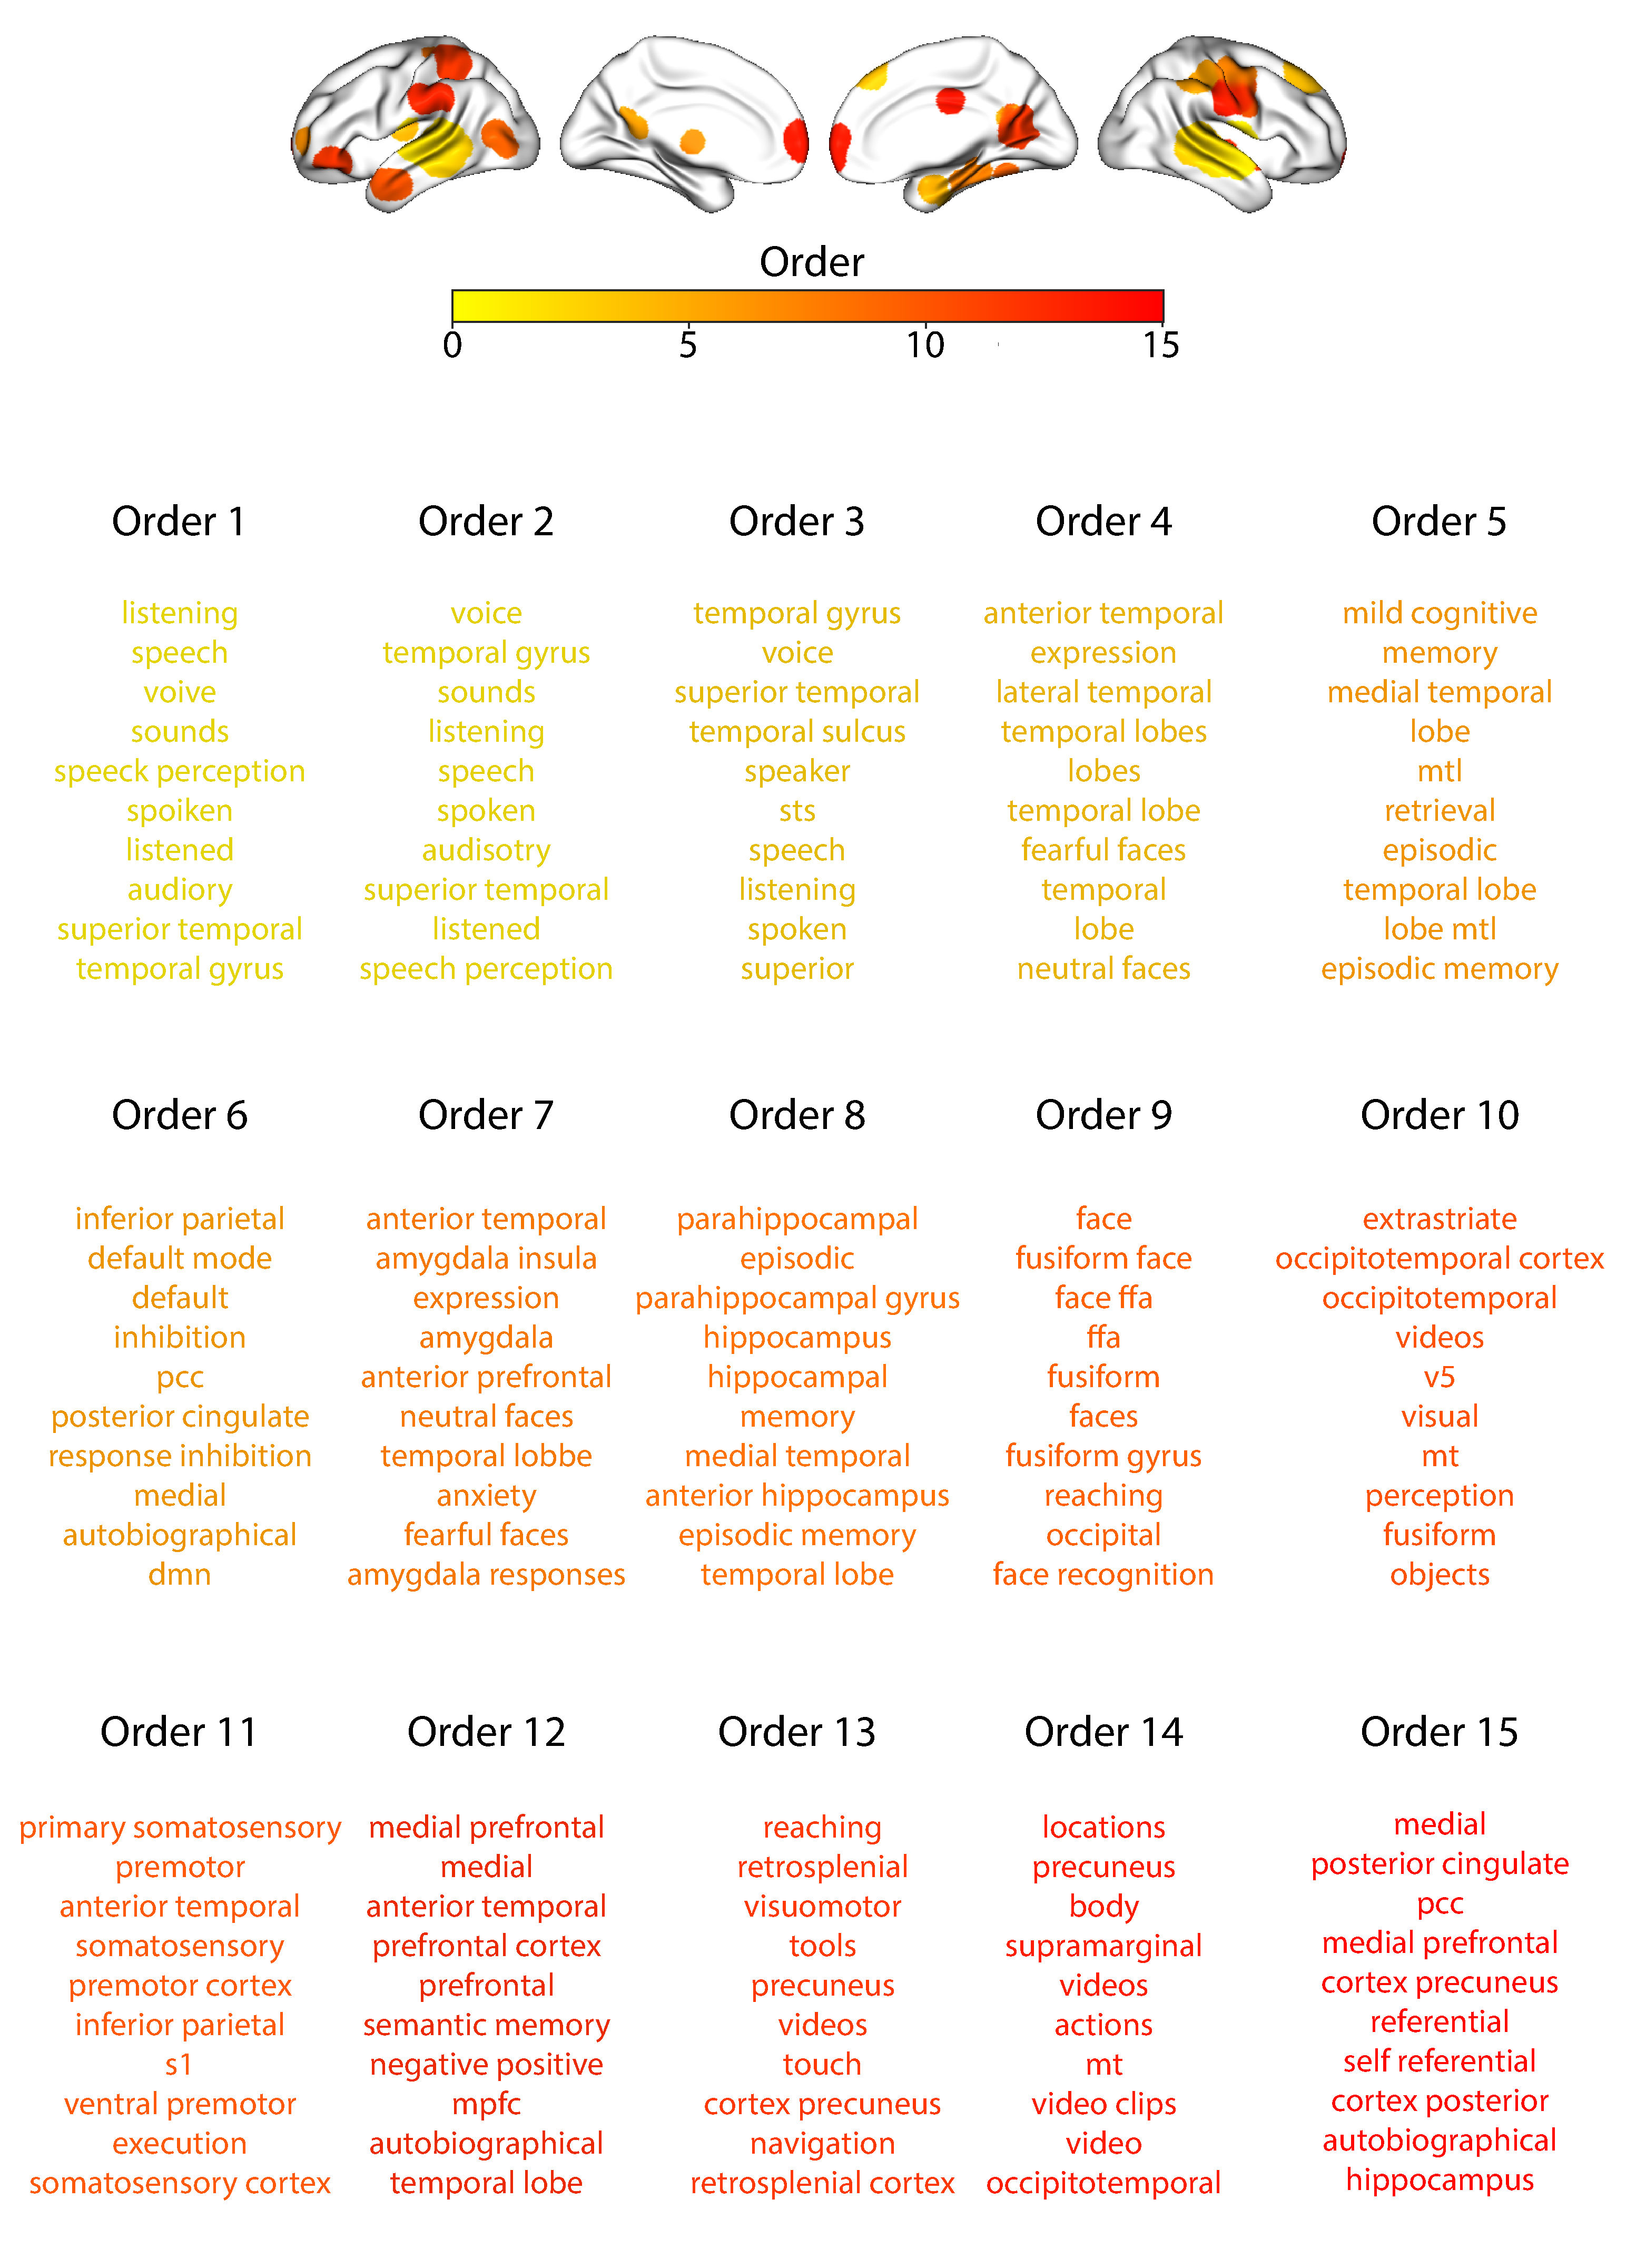
\includegraphics[width=\textwidth]{figs/supp_15_word}
\caption{\small \textbf{Top 10 terms associated with the endpoints of the
      strongest correlations for the word scrambled condition.}  Each color corresponds to orders 1-15 of
    inter-subject functional correlations for the word scrambled condition. The inflated brain plots
    display the locations of the endpoints of the 10 strongest
    (absolute value) correlations at each order, projected onto the
    cortical surface~\citep{CombEtal19}.  The lists of terms on the
    right display the top 10 Neurosynth terms~\citep{RubiEtal17}
    decoded from the corresponding brain maps for each order.}
\label{fig:word}
\end{figure}

\begin{figure}[p!]
\centering
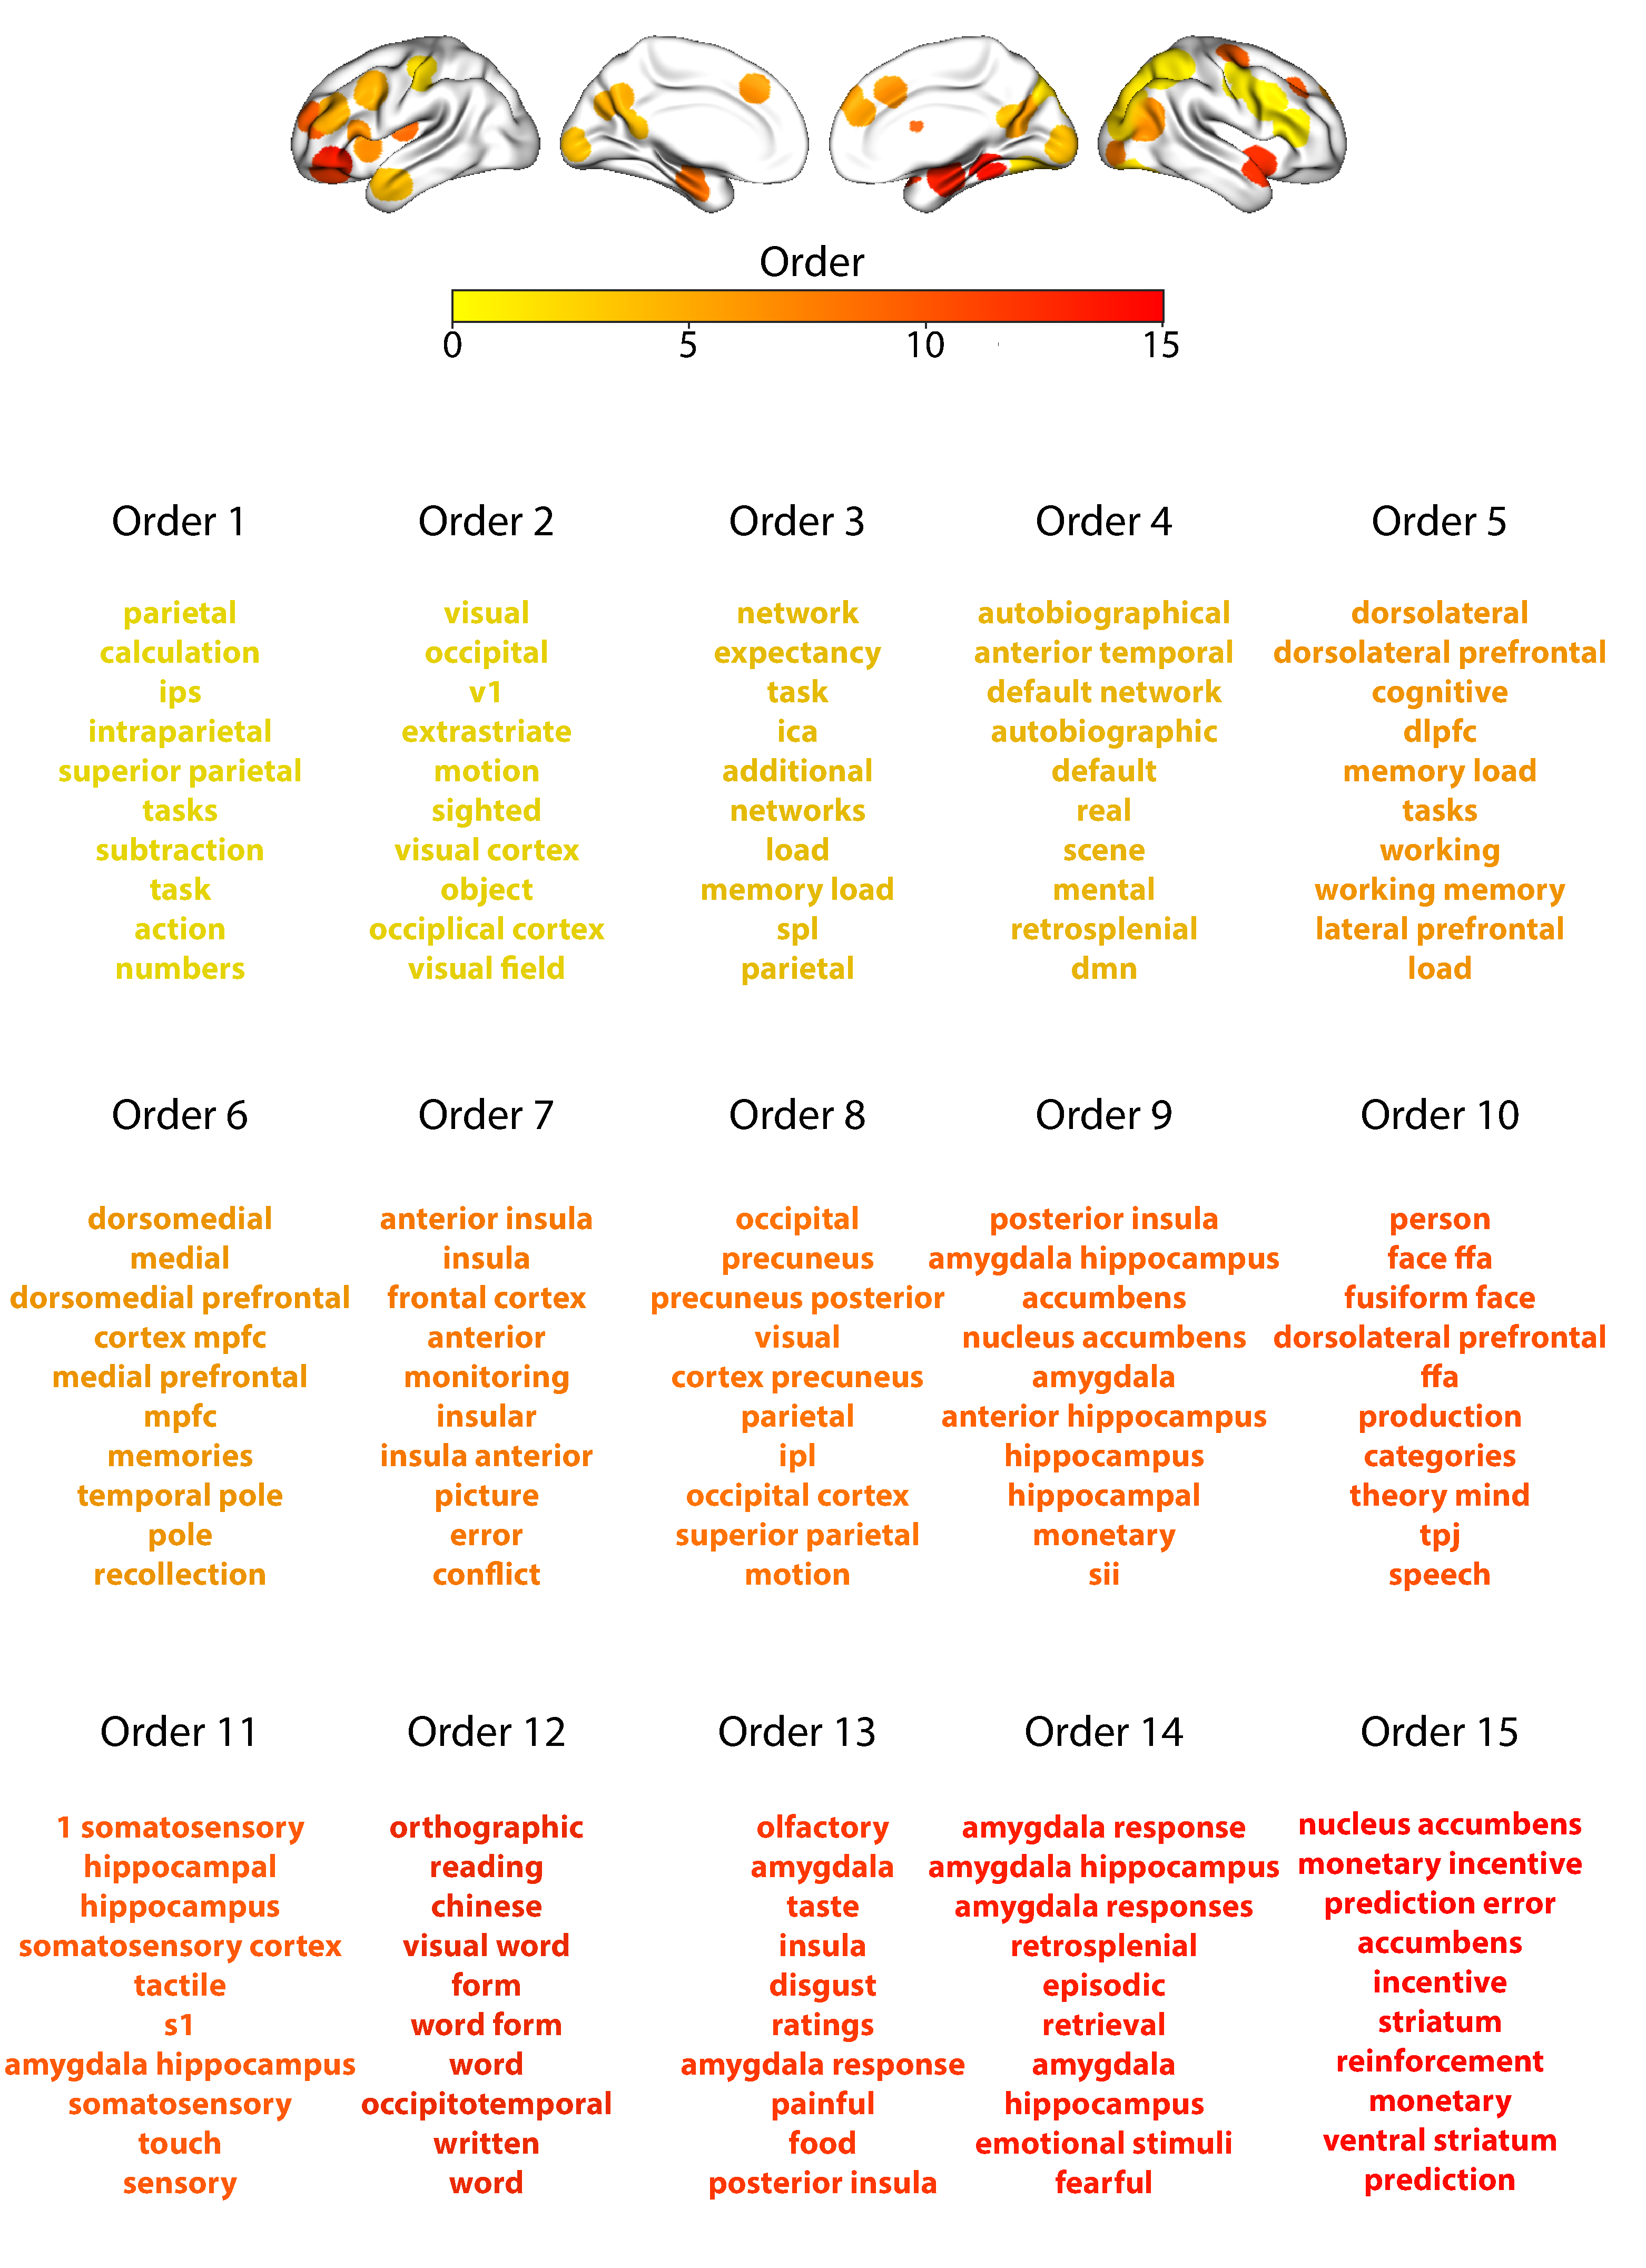
\includegraphics[width=\textwidth]{figs/supp_15_rest}
\caption{\small \textbf{Top 10 terms associated with the endpoints of the
      strongest correlations for the rest condition.}  Each color corresponds to orders 1-15 of
    inter-subject functional correlations for the rest condition. The inflated brain plots
    display the locations of the endpoints of the 10 strongest
    (absolute value) correlations at each order, projected onto the
    cortical surface~\citep{CombEtal19}.  The lists of terms on the
    right display the top 10 Neurosynth terms~\citep{RubiEtal17}
    decoded from the corresponding brain maps for each order.}
\label{fig:rest}
\end{figure}



%\section*{Participant-level figures referenced in the main text}

% Supporting information


\newpage
\renewcommand{\refname}{Supplemental references}
\bibliography{memlab}


\end{document}